\documentclass{article}

% if you need to pass options to natbib, use, e.g.:
% \PassOptionsToPackage{numbers, compress}{natbib}
% before loading nips_2017
%
% to avoid loading the natbib package, add option nonatbib:

\usepackage[nonatbib, final]{nips_2017}

% to compㅁle a camera-ready version, add the [final] option, e.g.:
\usepackage[utf8]{inputenc} % allow utf-8 input
\usepackage[T1]{fontenc}    % use 8-bit T1 fonts
\usepackage{hyperref}       % hyperlinks
\usepackage{url}            % simple URL typesetting
\usepackage{booktabs}       % professional-quality tables
\usepackage{amsfonts}       % blackboard math symbols
\usepackage{nicefrac}       % compact symbols for 1/2, etc.
\usepackage{microtype}      % microtypography
\usepackage{amsmath, amssymb, amsfonts, amsthm}
\usepackage[export]{adjustbox}
\usepackage{subcaption}
\usepackage[font=small]{caption}
\usepackage{todonotes}
\usepackage[]{algorithm2e}

% Some reference styles
\newcommand{\eref}[1]{(\ref{#1})}% Equation
\newcommand{\aref}[1]{Algorithm~\ref{#1}}% Algorithm
\newcommand{\sref}[1]{Section~\ref{#1}}% Section
\newcommand{\figref}[1]{Figure~\ref{#1}}% Figure
\newcommand{\tabref}[1]{Table~\ref{#1}}% Table

\DeclareMathOperator*{\argmax}{arg\,max}
\DeclareMathOperator*{\argmin}{arg\,min}
\bibliographystyle{ieeetr}

\title{Bayesian-Adaptive Deep Reinforcement Learning using Model Ensembles}

% The \author macro works with any number of authors. There are two
% commands used to separate the names and addresses of multiple
% authors: \And and \AND.
%
% Using \And between authors leaves it to LaTeX to determine where to
% break the lines. Using \AND forces a line break at that point. So,
% if LaTeX puts 3 of 4 authors names on the first line, and the last
% on the second line, try using \AND instead of \And before the third
% author name.

\author{
  Gilwoo Lee \\ \texttt{gilwoo@cs.uw.edu} \\
  %% examples of more authors
  \And
  Jeongseok Lee \\ \texttt{jslee02@cs.uw.edu} \\
  \And
  Brian Hou \\ \texttt{bhou@cs.uw.edu} \\
  \And
  Aditya Vamsikrishna \\ \texttt{adityavk@cs.uw.edu} \\
}

\begin{document}

\maketitle

    \begin{abstract}
    lalala abstract!
    \end{abstract}

\section{Introduction}
While reinforcement learning is capable of controlling complex autonomous systems, RL algorithms typically require huge amounts of data, can overfit to a particular task, or may learn brittle policies that are prone to disturbances. One of the main challenges that needs to be addressed is to train a policy that is robust to various model uncertainties and disturbances. In this project, we aim to address this challenge via an ensemble policy for Bayes-Adaptive Reinforcement Learning~\cite{ghavamzadeh2015bayesian}.

We model $b_\phi$ as a network capable of modeling evolving state change, e.g., Recurrent Neural Networks, or as a Bayes filter. At the low level, we plan to discretize $\Phi$ and have one actor-critic network per discretized value of $\phi$: each critic estimates $V^*(\cdot;\phi)$ and each actor has an optimal policy for a particular discretized value of $\pi^*(\cdot;\phi)$. Given $b_\phi$ and the set of value-function approximators, it is straightforward to compute (\ref{eq:barl}).

\section{Related Works}
Our work is closely related to QMDP~\cite{littman1995learning, karkus2017qmdp} which is an approximation for POMDP. QMDP approximates POMDP by assuming fully-observable MDP after 1-step, and approximating the Q-value at the current belief state $b(s)$ as $Q_a(b) =\sum_s b(s)Q_{\text{MDP}}(s, a)$. In our problem setup, we have a belief over the physics parameters $\phi$ of the MDP, $b(\phi)$, and we compute the policy $Q_a(s;b) = \sum_\phi b(\phi)Q_{\text{MDP}}(s,a;\phi)$.

The BAMDP formulation is also similar to POMDP formulation used in POMDP-lite~\cite{chen2016pomdp} which assumes that the hidden state variables are constant or only change deterministically. In our case, the hidden state variables correspond to the physics parameters $\phi$. The authors of POMDP-lite have shown that such formulation is ``equivalent to a set of fully observable Markov decision processes indexed by a hidden parameter''~\cite{chen2016pomdp}, which, in our case, is a discretization of $\phi$.

\newpage

\section{Bayes-Adaptive Reinforcement Learning}
\begin{figure*}[h!]
\begin{subfigure}[b]{0.3\columnwidth}
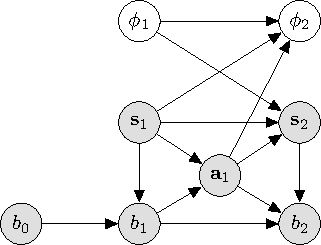
\includegraphics[width=\linewidth]{figs/model.pdf}
\caption{Graphical Model}
\end{subfigure}
\hfill
\begin{subfigure}[b]{0.65\columnwidth}
\missingfigure[figwidth=6cm]{Testing a long text string}
\caption{System structure}
\end{subfigure}
\end{figure*}

We assume that there exists a latent physics variable $\phi$ which determines the transition function of the underlying MDP, i.e., the transition function  $P(s',\phi' |s, \phi, a)$ is now a function of state, action, and $\phi$. We would like to learn a policy which maximizes the long term reward given $\phi$. Formally, this is called a Bayes-Adaptive MDP~\cite{ghavamzadeh2015bayesian, ross2008bayes, guez2012efficient}, defined by a tuple $\langle \mathcal{S}', \mathcal{A}, P, P_0, R \rangle$ where
\begin{itemize}
\item $\mathcal{S'} = \mathcal{S}\times \Phi$ is the set of hyper-states (states, physics variable),
\item $\mathcal{A}$ is the set of actions,
\item $P(s',\phi'|s, \phi, a)$ is the transition function between hyper-states, conditioned
on action $a$ being taken in hyper-state $(s, \phi)$,
\item $P_0\in \mathcal{P}(\mathcal{S} \times \Phi)$ combines the initial distribution over hyper-states,
\item $R(s, \phi, a)$ represents the reward obtained when action $a$ is
taken in hyper-state $(s,\phi)$.
\end{itemize}

We would like to find the Bayes-optimal policy for the following Bellman equaton:
\begin{equation}\label{eq:rl}
V^*(b, s) = \max_a \bigg\{R(b, s, a) + \gamma \sum_{s'}P(s'|b, s, a)V^*(b', s') \bigg\}.
\end{equation}
where $b$ is the belief over the set of latent physics parameters $\phi \in \Phi$.

We make a simplification to the BARL formulation. We assume that the latent variable $\phi$ is either constant or the rate of change is slow enough that approximating the long-term value with a determinized $\phi$ is a reasonable short-term approximation for choosing one-step action, i.e. we can treat $V^*(s_t, \phi_t) \approx V^*(s_t, \phi_{t:\infty})$ for the purpose of one-step Bellman update.

This assumption allows us to simplify BARL with an ensemble policy learning method. At a high level, we have a network that updates the \emph{belief} of the physics parameters at time $t$,
\begin{align*}
b(\phi_t) = P(\phi_t|s_{t-1}, \phi_{t-1}, a_{t-1})
\end{align*}
which is then used to compute the best policy from an ensemble of $\phi$-dependent optimal policies, i.e., $\pi^*(\cdot;\phi)$ and $V^*(\cdot;\phi)$ are computed with typical RL algorithms for MDPs. Then the remaining task is to compute the one-step best action $a$:
\begin{align}\label{eq:barl}
 a^* &= \argmax_{a} \mathbb{E}_{\phi \sim b(\phi)} \bigg[R(s, a, \phi) + \gamma \sum_{s', \phi'}P(s',\phi'|s, \phi, a)V^{*'}(s', \phi') \bigg].
\end{align}

\section{Bayes-Adaptive Policy Network}

TODO: Explain how the system works (input to the network, etc.)

\begin{algorithm}[t!]
 \KwData{this text}
 \KwResult{how to write algorithm with \LaTeX2e }
 initialization\;
 \While{not at end of this document}{
  read current\;
  \eIf{understand}{
   go to next section\;
   current section becomes this one\;
   }{
   go back to the beginning of current section\;
  }
 }
 \caption{TODO: write the algoruthm. (Change this to a prettier algorithm package)}
\end{algorithm}

\section{Experiments}

We have setup a set of simulated examples and a set of RL algorithms to be utilized in our ensemble approach. For simulated examples, we have the following agents: \textbf{ant, reacher, swimmer, half-cheetah}, each with a predefined reward function defined similar to those given by OpenAI Gym~\cite{openai}. We are utilizing TRPO~\cite{trpo}, VPG, DDPG~\cite{ddpg} provide by \texttt{rllab}~\cite{duan2016benchmarking} as a set of algorithms to be utilized in our ensemble approach. In addition, we plan to implement PPO and a PID controller for RACECAR.

Our algorithm will be compared against two classes of algorithms: (1) sample-based algorithms which chooses an MDP and commit to this policy for a fixed horizon, and (2) ensemble algorithms which train a policy over an ensemble of MDP models. A greedy algorithm which chooses the maximum-likely MDP, or one that samples from a posterior distribution of MDPs given previous observations (e.g. Posterior Sampling Reinforcement Learning \cite{psrl}) would fall into the former, and EPOpt\cite{rajeswaran2016epopt} and Ensemble-CIO~\cite{ensemble-cio} would fall into the latter.

We are currently in the process of setting up baseline algorithms which may be used for direct comparison or as internal policy update algorithms for each of MDP in our algorithm.

\newpage
\begin{figure*}[t!]
\begin{centering}
\begin{subfigure}[b]{0.3\columnwidth}
\adjincludegraphics[height=3cm,trim={{.6\width} {0.4\height} {0.15\width} {0.35\height}},clip=true]{figs/keyframes/cheetah/cheetah_nominal.png}
\caption{Nominal}
\end{subfigure}
\begin{subfigure}[b]{0.3\columnwidth}
\adjincludegraphics[height=3cm,trim={{.5\width} {0.4\height} {0.25\width} {0.35\height}},clip=true]{figs/keyframes/cheetah/cheetah_170_92.png}
\caption{Key frames}
\end{subfigure}
\begin{subfigure}[b]{0.3\columnwidth}
\adjincludegraphics[height=3cm,trim={{.5\width} {0.4\height} {0.25\width} {0.35\height}},clip=true]{figs/keyframes/cheetah/cheetah_150_150.png}
\caption{Key frames}
\end{subfigure}
\end{centering}
\caption{Keyframes from rollouts on various MDPs. The universal policy network learns to use different policies on different MDPs.}
\end{figure*}


\newpage
\begin{figure*}[t!]
\begin{centering}
\begin{subfigure}[b]{0.38\columnwidth}
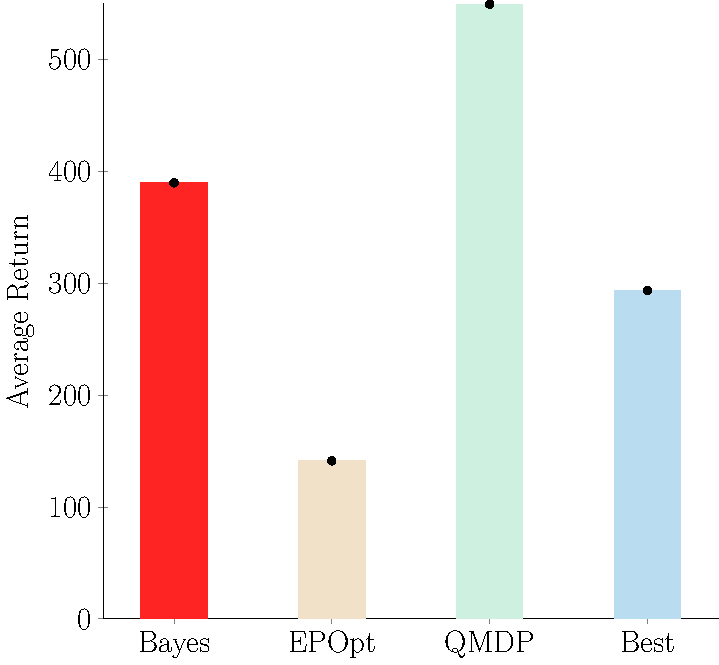
\includegraphics[width=\linewidth]{figs/cheetah_nominal_comparison.pdf}
\subcaption{Return on a sampled MDP}
\end{subfigure}
~
\begin{subfigure}[b]{0.38\columnwidth}
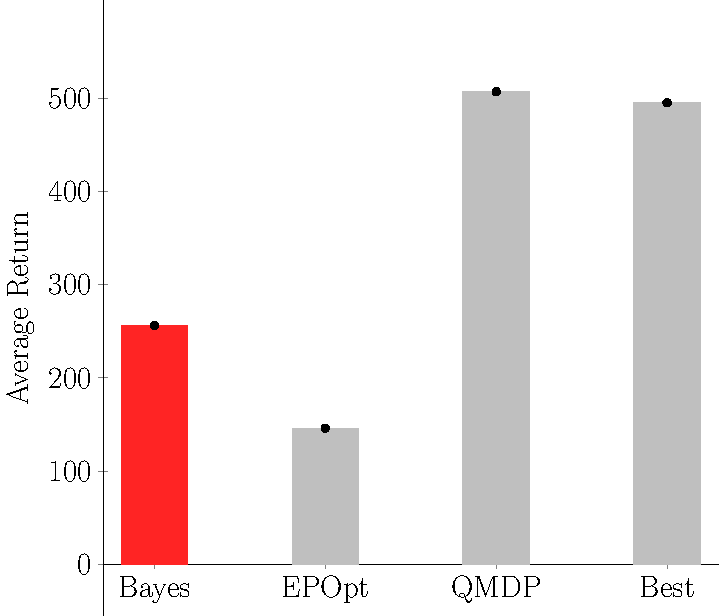
\includegraphics[width=\linewidth]{figs/cheetah_env_comparison.pdf}
\subcaption{Return on one of the chosen MDPs}
\end{subfigure}
~
\begin{subfigure}[b]{0.20\columnwidth}
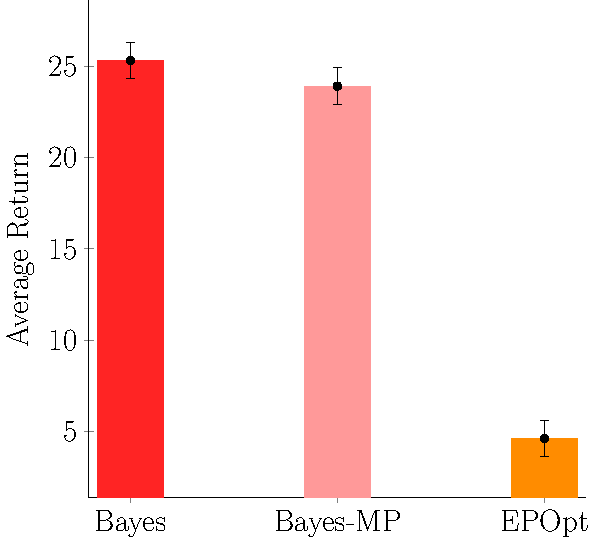
\includegraphics[width=\linewidth]{figs/ant_average.pdf}
\subcaption{Average return}
\end{subfigure}
\end{centering}
\caption{Return on sampled and prechosen MDPs. BARL is better than EPOpt. On average across K pre-chosen MDPs, it outperforms EPOpt by a large margin. TODO: remove BMP.}
\end{figure*}

\begin{figure*}[t!]
\begin{centering}
\begin{subfigure}[b]{0.38\columnwidth}
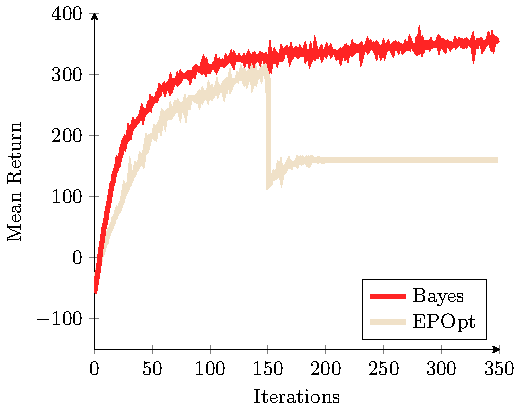
\includegraphics[width=\linewidth]{figs/cheetah_training_curves.pdf}
\subcaption{Return on a sampled MDP}
\end{subfigure}
~
\begin{subfigure}[b]{0.38\columnwidth}
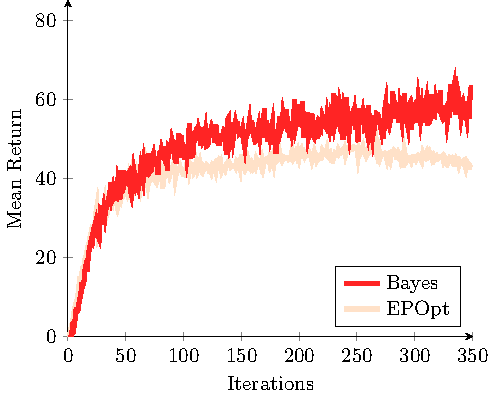
\includegraphics[width=\linewidth]{figs/swimmer_training_curves.pdf}
\end{subfigure}
\end{centering}
\caption{Training curves}
\end{figure*}



\newpage
\begin{figure*}[t!]
\begin{centering}
\begin{subfigure}[b]{0.3\columnwidth}
\adjincludegraphics[height=3cm,trim={{.4\width} {0.42\height} {0.35\width} {0.33\height}},clip=true]{figs/keyframes/ant/ant_nominal_18.png}
\caption{Nominal}
\end{subfigure}
\hfill
\begin{subfigure}[b]{0.3\columnwidth}
\adjincludegraphics[height=3cm,trim={{.4\width} {0.42\height} {0.35\width} {0.33\height}},clip=true]{figs/keyframes/ant/ant_120_19.png}
\caption{Key frames}
\end{subfigure}
\hfill
\begin{subfigure}[b]{0.3\columnwidth}
\adjincludegraphics[height=3cm,trim={{.6\width} {0.34\height} {0.15\width} {0.41\height}},clip=true]{figs/keyframes/ant/ant_140_87.png}
\caption{Key frames}
\end{subfigure}
\vfill
\begin{subfigure}[b]{0.3\columnwidth}
\adjincludegraphics[height=3cm,trim={{.55\width} {0.34\height} {0.20\width} {0.41\height}},clip=true]{figs/keyframes/swimmer/swimmer_nominal.png}
\caption{Nominal}
\end{subfigure}
\hfill
\begin{subfigure}[b]{0.3\columnwidth}
\adjincludegraphics[height=3cm,trim={{.55\width} {0.40\height} {0.20\width} {0.35\height}},clip=true]{figs/keyframes/swimmer/swimmer_20_12.png}
\caption{Key frames}
\end{subfigure}
\hfill
\begin{subfigure}[b]{0.3\columnwidth}
\adjincludegraphics[height=3cm,trim={{.35\width} 0 {0.40\width} {0.55\height}},clip=true]{figs/keyframes/swimmer/swimmer_40_157.png}
\caption{Key frames}
\end{subfigure}
\caption{Keyframes from rollouts on various MDPs. Some of the MDPs are gemeotrically significatnly differnt that they require drastically different policies to achieve optimal returns.}
\end{centering}
\end{figure*}

\bibliography{intuitive_physics}

\end{document}
